\documentclass[conference]{IEEEtran}
\IEEEoverridecommandlockouts
\usepackage{cite}
\usepackage{amsmath,amssymb,amsfonts}
\usepackage{algorithmic}
\usepackage{algorithm}
\usepackage{graphicx}
\usepackage{textcomp}
\usepackage{xcolor}
\usepackage{booktabs}
\usepackage{multirow}
\usepackage{url}
\usepackage{listings}
\usepackage{subcaption}
\usepackage{tikz}
\usetikzlibrary{shapes.geometric, arrows.meta, positioning, fit, backgrounds, calc}

\newcommand{\todo}[1]{\textcolor{red}{\textbf{TODO:} #1}}
\newcommand{\elaine}[1]{\textcolor{violet}{\textbf{EW:} #1}}

\lstset{
  basicstyle=\ttfamily\scriptsize,
  breaklines=true,
  frame=single,
  numbers=left,
  numberstyle=\tiny,
  xleftmargin=2em,
  framexleftmargin=1.5em,
  captionpos=b
}

\def\BibTeX{{\rm B\kern-.05em{\sc i\kern-.025em b}\kern-.08em
    T\kern-.1667em\lower.7ex\hbox{E}\kern-.125emX}}

\begin{document}

\title{Agentic MLIR-to-QIR Translation with Verification: A Hybrid Deterministic and LLM Approach
\thanks{This manuscript has been authored by UT-Battelle, LLC, under Contract No. DEAC0500OR22725 with the U.S. Department of Energy. The United States Government
retains and the publisher, by accepting the article for publication, acknowledges that
the United States Government retains a non-exclusive, paid-up, irrevocable, worldwide license to publish or reproduce the published form of this manuscript, or allow
others to do so, for the United States Government purposes. The Department of
Energy will provide public access to these results of federally sponsored research in
accordance with the DOE Public Access Plan.}}

\author{
\IEEEauthorblockN{Sharmin Afrose, Vicente Leyton-Ortega, Narasinga Rao Miniskar, Elaine Wong, Travis S. Humble}
\IEEEauthorblockA{\textit{Oak Ridge National Laboratory}, Oak Ridge, TN, USA \\
\{afroses, leytonortheva, miniskarnr, wongey, humblets\}@ornl.gov}
}

\maketitle

\begin{abstract}
We present a hybrid system for translating MLIR quantum circuits to QIR that combines deterministic compiler techniques with large language model (LLM) agents. The system implements three translation paths: deterministic for recognized dialects (Catalyst and Quake), fully agentic for unseen dialects, and a repair path where LLM agents correct deterministic output that fails verification. A dual-backend verification pipeline independently executes source MLIR and generated QIR on separate simulators, comparing output distributions via total variation distance (TVD). A guardrail-assembler pattern recovers valid QIR from structurally incomplete LLM output, and context engineering replaces retrieval-augmented generation for smaller models. On a 39-circuit benchmark spanning three dialects (including an unseen fault-tolerant quantum computing dialect) and scaling from 5 to 100 qubits, the deterministic path achieves 98.6\% gate-level correctness (71/72 circuit-dialect pairs) with TVD similarity averaging 97.9--99.3\% across simulable circuits, and cross-dialect evaluation on 14 matched Catalyst--Quake pairs confirms gate-level equivalence. For the unseen FTQC dialect, the agentic path produces valid logical-level QIR on the first iteration, demonstrating the system's extensibility to dialects beyond its deterministic parser.
\end{abstract}

\begin{IEEEkeywords}
quantum intermediate representation, MLIR, QIR, large language models, multi-agent systems, quantum circuit translation, verification
\end{IEEEkeywords}

\section{Introduction}

Quantum computing is undergoing rapid diversification in both hardware platforms and software toolchains~\cite{preskill2018quantum, heim2020quantum}. As hardware vendors and research groups introduce competing frameworks, including IBM Qiskit~\cite{javadi2024qiskit}, Google Cirq~\cite{cirq2024}, Microsoft Q\#~\cite{svore2018qsharp}, Xanadu PennyLane~\cite{bergholm2022pennylane}, and NVIDIA CUDA Quantum~\cite{kim2023cudaquantum}, the quantum software stack has grown increasingly fragmented. Each framework defines its own intermediate representation (IR) for expressing quantum circuits, creating a significant interoperability barrier: circuits authored in one framework cannot be readily executed on another platform's backend without manual or semi-automated translation~\cite{cardama2025review}.

The Multi-Level Intermediate Representation (MLIR) framework~\cite{lattner2021mlir}, originally developed to address the ``end of Moore's law'' challenges in classical compiler infrastructure, has emerged as a unifying substrate for quantum compilation. Several quantum projects have adopted MLIR's extensible dialect mechanism to define domain-specific representations: PennyLane Catalyst~\cite{ittah2024catalyst} introduces a quantum dialect for just-in-time compilation of hybrid quantum-classical programs, while CUDA Quantum defines the Quake dialect for GPU-accelerated quantum simulation~\cite{kim2023cudaquantum}. McCaskey and Nguyen~\cite{mccaskey2021mlirdialect} first demonstrated the viability of MLIR dialects for quantum assembly languages, and recent work by Hopf et al.~\cite{hopf2026integrating} has explored integrating multiple quantum tools within the MLIR ecosystem.

On the execution side, the Quantum Intermediate Representation (QIR)~\cite{qirspec2021}, built atop LLVM IR~\cite{lattner2004llvm}, has gained traction as a portable compilation target. QIR defines a standard set of quantum intrinsics (qubit allocation, gate application, measurement, and result recording) that multiple simulators and hardware backends can consume, making it a natural hub for cross-framework interoperability. However, bridging the gap between MLIR quantum dialects and QIR currently requires hand-written compiler passes for each source dialect, an approach that scales poorly as new dialects appear~\cite{cardama2025review, hopf2026integrating}.

Recent advances in large language models (LLMs) have shown strong competence in code generation~\cite{chen2021codex, li2022alphacode} and code translation~\cite{szafraniec2023code} tasks. Specialized models such as Code Llama~\cite{roziere2023codellama} and GPT-4~\cite{achiam2023gpt4} have shown the ability to translate between programming languages, while domain-specific efforts like the Qiskit Code Assistant~\cite{dupuis2024qiskitassistant} and Agent-Q~\cite{jern2025agentq} have begun applying LLMs to quantum code generation. The emergence of multi-agent orchestration frameworks~\cite{hong2024crewai, wu2023autogen} and structured reasoning paradigms such as ReAct~\cite{yao2023react} and Reflexion~\cite{shinn2023reflexion} further suggest that agentic systems can tackle complex, multi-step code transformation tasks that exceed the capability of single-pass generation.

However, applying LLMs to quantum IR translation presents unique challenges distinct from general-purpose code translation. Quantum IR has strict syntactic requirements (e.g., LLVM type annotations, function declaration ordering), subtle semantic constraints (e.g., qubit pointer indexing conventions, measurement recording protocols), and zero tolerance for hallucinated operations that would alter the circuit's quantum behavior. In practice, smaller open-weight models (8B--13B parameters) that are practical for local deployment frequently produce structurally incomplete output, omitting scaffolding elements required for valid QIR while preserving the correct gate sequence.

In this paper, we present an agentic translation system that addresses these challenges through a hybrid architecture combining deterministic parsing with LLM-based translation and iterative repair. Our principal contributions are:

\begin{enumerate}
    \item A \textbf{three-path translation strategy} that dynamically selects between deterministic, fully agentic, and hybrid repair modes based on dialect recognition and verification outcomes.
    \item A \textbf{dual-backend verification pipeline} that independently executes the source MLIR and generated QIR on separate quantum simulators (PennyLane Catalyst, CUDA Quantum, or other backends via an extensible registry) and QIR Runner, comparing output probability distributions via total variation distance (TVD).
    \item A \textbf{guardrail-assembler pattern} that recovers valid QIR from structurally incomplete LLM output by extracting gate operations and deterministically reassembling them using validated templates.
    \item A \textbf{context engineering} approach that injects gate mappings and QIR templates directly into agent prompts, eliminating the failure modes associated with retrieval-augmented generation (RAG) on smaller models.
\end{enumerate}

The remainder of this paper is organized as follows. Section~\ref{sec:related} reviews related work in quantum IR translation and LLM-based code generation. Section~\ref{sec:methodology} presents the system architecture and methodology. Section~\ref{sec:experiments} describes the experimental setup and evaluation metrics. Section~\ref{sec:results} reports experimental results. Section~\ref{sec:discussion} discusses findings and limitations, and Section~\ref{sec:conclusion} concludes with directions for future work.


\section{Related Work}\label{sec:related}

We organize the related work into four areas: quantum IRs, MLIR-based quantum compilation, LLM-driven code generation and translation, and verification of quantum circuit transformations.

\subsection{Quantum Intermediate Representations}

The proliferation of quantum hardware platforms has motivated the development of multiple intermediate representations that serve as abstraction layers between high-level quantum programs and low-level control pulses. OpenQASM~3~\cite{cross2022openqasm3}, developed by IBM, extends the original OpenQASM language with classical control flow, subroutines, and timing primitives, establishing itself as a widely adopted circuit-level interchange format. The QIR specification~\cite{qirspec2021}, proposed by the QIR Alliance, takes a complementary approach by encoding quantum operations as intrinsic function calls within LLVM IR~\cite{lattner2004llvm}, thereby inheriting LLVM's mature optimization infrastructure and enabling interoperability with classical compilation pipelines.

Cardama et al.~\cite{cardama2025review} provide a comprehensive survey of quantum IRs, comparing representations including QIR, QSSA, and various MLIR-based dialects along dimensions of expressiveness, optimization support, and tool ecosystem maturity. Ittah et al.~\cite{ittah2022qiro} proposed QIRO, an SSA-based quantum program representation built on MLIR that supports dataflow-driven optimizations analogous to those in classical compilers. Luo and Zhao~\cite{singhal2024formal} contributed a formalization of quantum intermediate representations, analyzing type-safety properties and demonstrating that well-typed quantum IR programs preserve qubit linearity and measurement consistency. These efforts collectively establish the theoretical foundations upon which our translation system operates, but none address the problem of automated cross-dialect translation.

\subsection{MLIR for Quantum Compilation}

The adoption of MLIR~\cite{lattner2021mlir} for quantum computing was pioneered by McCaskey and Nguyen~\cite{mccaskey2021mlirdialect}, who demonstrated that MLIR's progressive lowering mechanism and extensible dialect system are well-suited for expressing quantum operations at multiple levels of abstraction. This foundational insight has been realized in two major quantum compilation frameworks.

PennyLane Catalyst~\cite{ittah2024catalyst} introduces a quantum dialect within MLIR that enables just-in-time compilation of hybrid quantum-classical programs. Catalyst's dialect defines operations such as \texttt{quantum.alloc}, \texttt{quantum.custom}, and \texttt{quantum.measure} that map directly to quantum gate semantics, and the compiler lowers these progressively through MLIR's pass infrastructure to executable code. CUDA Quantum~\cite{kim2023cudaquantum} defines the Quake dialect, which follows a similar multi-level approach but targets NVIDIA's GPU-accelerated quantum simulation backends and can lower to QIR as a compilation target.

Recent work by Hopf et al.~\cite{hopf2026integrating} has explored integrating PennyLane Catalyst with the Munich Quantum Toolkit (MQT) via MLIR, demonstrating that the MLIR ecosystem can serve as a bridge between independently developed quantum tools. While these efforts advance intra-MLIR interoperability, they rely on manually authored compiler passes for each dialect pair, the very scalability limitation our agentic approach is designed to overcome.

\subsection{LLM-Driven Code Generation and Translation}

Large language models have achieved strong performance on code generation benchmarks~\cite{chen2021codex, li2022alphacode, austin2021program}, with models such as GPT-4~\cite{achiam2023gpt4} and Code Llama~\cite{roziere2023codellama} demonstrating the ability to produce functionally correct programs from natural language specifications. Szafraniec et al.~\cite{szafraniec2023code} showed that incorporating compiler intermediate representations (specifically LLVM IR) as a pivot improves neural code translation between languages, a finding directly relevant to our MLIR-to-QIR translation task.

In the quantum domain, Dupuis et al.~\cite{dupuis2024qiskitassistant} developed the Qiskit Code Assistant by fine-tuning Granite LLMs on quantum computing code, achieving improved performance on Qiskit-specific generation tasks. Jern et al.~\cite{jern2025agentq} proposed Agent-Q, which applies fine-tuned LLMs to quantum circuit generation and optimization in OpenQASM~3 format. However, both of these efforts target high-level quantum SDKs (Qiskit Python or OpenQASM) rather than low-level LLVM-based representations like QIR, which imposes substantially stricter syntactic and structural requirements.

A complementary line of work has explored machine learning for classical compiler optimization. Cummins et al.~\cite{cummins2020programl} introduced ProGraML, a graph-based deep learning framework for program optimization using LLVM IR as the representation, demonstrating that neural models can reason about compiler IRs. Our work differs in that we use LLMs for cross-IR \emph{translation} rather than optimization within a single IR, and we operate on quantum-extended LLVM IR where correctness is defined by quantum mechanical equivalence of output distributions.

\subsection{Agentic AI for Software Engineering}

The concept of LLM-based agents that combine reasoning with tool use has been formalized by the ReAct paradigm~\cite{yao2023react}, which interleaves chain-of-thought reasoning~\cite{wei2022chainofthought} with actions such as code execution and web search. Shinn et al.~\cite{shinn2023reflexion} extended this approach with Reflexion, which enables agents to improve through verbal self-reflection on execution feedback, a pattern closely related to our iterative verification-feedback loop.

Multi-agent frameworks such as AutoGen~\cite{wu2023autogen} and CrewAI~\cite{hong2024crewai} provide infrastructure for orchestrating multiple specialized agents on complex tasks. Wang et al.~\cite{wang2024agentsurvey} survey the application of LLM-based agents to software engineering, identifying code generation, testing, and debugging as areas of demonstrated success. Our system extends these patterns to quantum compiler engineering, using a translation agent that generates QIR and a verification pipeline that provides structured feedback for iterative repair. The use of context engineering over retrieval-augmented generation (RAG)~\cite{lewis2020rag} is a pragmatic adaptation to the failure modes we observed with smaller models.

\subsection{Quantum Circuit Verification}

Verifying the correctness of quantum circuit transformations is a recognized challenge in quantum compilation~\cite{karuppasamy2025comprehensive}. Bauer-Marquart et al.~\cite{bauer2023symqv} proposed symQV, a symbolic verification approach that proves equivalence of quantum programs through automated theorem proving. While formally rigorous, symbolic approaches face scalability limitations for circuits with many qubits or complex classical control flow.

Simulation-based verification offers a complementary approach: by executing both the original and transformed circuits on quantum simulators and comparing output distributions, one can detect semantic discrepancies without requiring formal proofs. Total variation distance (TVD) is a standard metric for comparing probability distributions in quantum information theory~\cite{nielsen2010quantum} and provides a symmetric, bounded measure of distributional agreement. Our dual-backend pipeline implements this simulation-based approach with the additional rigor of executing the source MLIR and target QIR on \emph{independent} backends, thereby avoiding shared-mode failures that could mask translation errors.

Table~\ref{tab:comparison} positions our work relative to existing quantum translation and code generation approaches.

\begin{table*}[t]
\centering
\caption{Comparison of approaches to quantum code translation and generation. Our system uniquely combines LLM-based translation with dual-backend simulation verification and support for multiple MLIR dialects.}
\label{tab:comparison}
\renewcommand{\arraystretch}{1.15}
\begin{tabular}{@{}lcccccc@{}}
\toprule
\textbf{System} & \textbf{Source} & \textbf{Target} & \textbf{LLM-Based} & \textbf{Multi-Agent} & \textbf{Sim. Verification} & \textbf{Extensible to New Dialects} \\
\midrule
Catalyst Compiler~\cite{ittah2024catalyst}        & MLIR (Catalyst) & Machine code & No  & No  & No  & No  \\
CUDA Quantum~\cite{kim2023cudaquantum}             & MLIR (Quake)    & QIR          & No  & No  & No  & No  \\
Qiskit Code Assistant~\cite{dupuis2024qiskitassistant} & NL / Code   & Qiskit Python & Yes & No  & No  & N/A \\
Agent-Q~\cite{jern2025agentq}                      & NL              & OpenQASM 3   & Yes & No  & Yes & N/A \\
Hopf et al.~\cite{hopf2026integrating}             & MLIR            & MLIR         & No  & No  & No  & Limited \\
\textbf{This work}                                  & MLIR (any)      & QIR          & Hybrid & Yes & \textbf{Dual-backend} & \textbf{Yes} \\
\bottomrule
\end{tabular}
\end{table*}


\section{Methodology}\label{sec:methodology}

This section presents the architecture and algorithms of the agentic MLIR-to-QIR translation system. The system consists of four principal components: dialect-aware parsing, multi-path translation, dual-backend verification, and an LLM output guardrail with deterministic reassembly. Fig.~\ref{fig:architecture} provides an overview of the system architecture and the interaction between components.


% =============================================
% TikZ Architecture Diagram
% =============================================
\begin{figure*}[t]
\centering
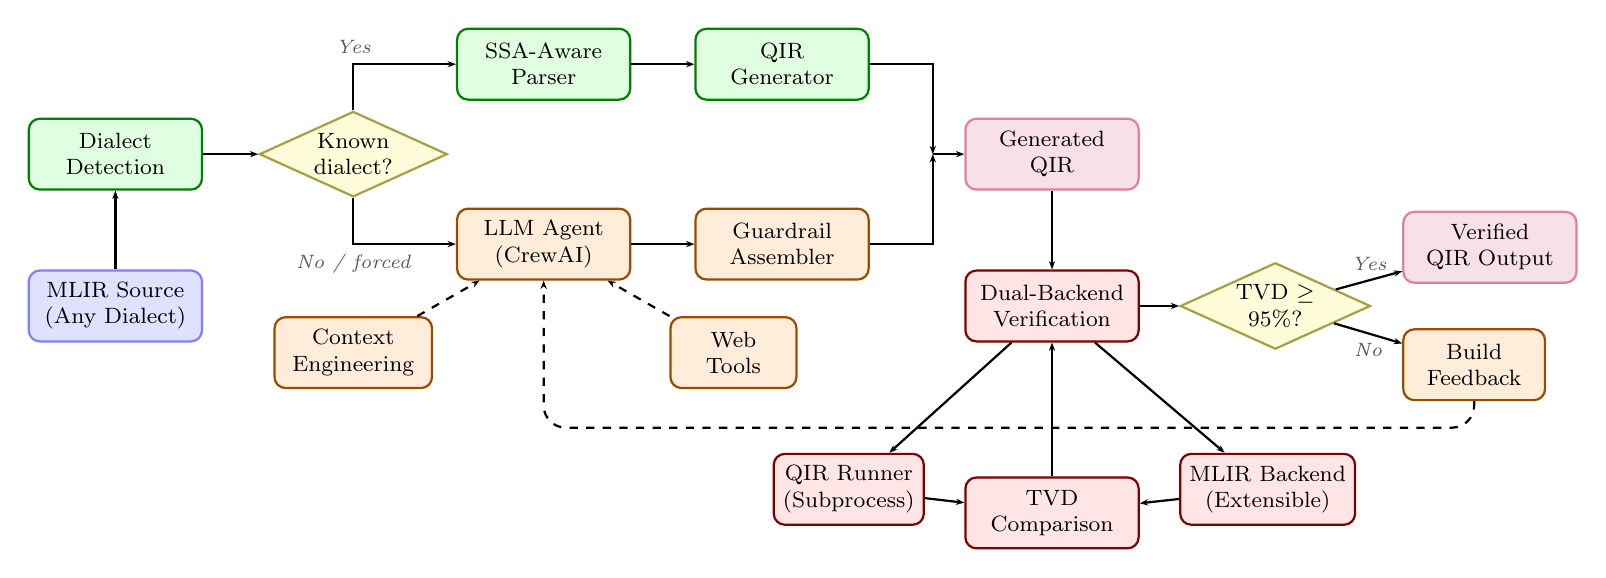
\begin{tikzpicture}[
    node distance=0.6cm and 0.8cm,
    box/.style={draw, rounded corners, minimum height=0.9cm, minimum width=2.2cm, align=center, font=\footnotesize},
    input/.style={box, fill=blue!12, draw=blue!50, thick},
    det/.style={box, fill=green!12, draw=green!50!black, thick},
    agent/.style={box, fill=orange!15, draw=orange!60!black, thick},
    verify/.style={box, fill=red!10, draw=red!50!black, thick},
    output/.style={box, fill=purple!12, draw=purple!50, thick},
    decision/.style={diamond, draw, thick, fill=yellow!15, draw=yellow!60!black, aspect=2.2, inner sep=1pt, font=\footnotesize, align=center},
    arrow/.style={-{Stealth[length=3pt]}, thick},
    dasharrow/.style={-{Stealth[length=3pt]}, thick, dashed},
    label/.style={font=\scriptsize\itshape, text=gray!70!black},
]

% Input
\node[input] (mlir) {MLIR Source\\(Any Dialect)};

% Dialect Detection
\node[det, above=1.0cm of mlir] (detect) {Dialect\\Detection};

% Decision
\node[decision, right=0.7cm of detect] (known) {Known\\dialect?};

% Path 1: Deterministic
\node[det, above right=0.4cm and 0.7cm of known] (parser) {SSA-Aware\\Parser};
\node[det, right=0.8cm of parser] (qirgen) {QIR\\Generator};

% Path 2: Agentic
\node[agent, below right=0.4cm and 0.7cm of known] (llmagent) {LLM Agent\\(CrewAI)};

% Context Engineering & Web Tools (below agent)
\node[agent, below=1.5cm of known, minimum width=2.0cm] (context) {Context\\Engineering};
\node[agent, right=3cm of context, minimum width=1.6cm] (webtool) {Web\\Tools};

% Guardrail
\node[agent, right=0.8cm of llmagent] (guardrail) {Guardrail\\Assembler};

% Merge point
\node[coordinate, right=0.8cm of qirgen] (merge1) {};
\node[coordinate, right=0.8cm of guardrail] (merge2) {};
\node[coordinate] at ($(merge1)!0.5!(merge2)$) (mergepoint) {};
\node[output, right=0.4cm of mergepoint] (qir) {Generated\\QIR};

% Verification Pipeline
\node[verify, below=1.0cm of qir] (verifbox) {Dual-Backend\\Verification};

% Two backends inside verification (stacked below)
\node[verify, below left=1.4cm and 0.5cm of verifbox, minimum width=1.8cm] (qirrun) {QIR Runner\\(Subprocess)};
\node[verify, below right=1.4cm and 0.5cm of verifbox, minimum width=1.8cm] (catrun) {MLIR Backend\\(Extensible)};

% TVD
\node[verify, below=0.5cm of verifbox, yshift=-1.2cm] (tvd) {TVD\\Comparison};

% Decision: Pass?
\node[decision, right=0.5cm of verifbox] (pass) {TVD $\geq$\\95\%?};

% Output
\node[output, above right=0.0cm and 1.0cm of pass] (success) {Verified\\QIR Output};
% Feedback loop
\node[agent, below right=0.0cm and 1.0cm of pass, minimum width=1.8cm] (feedback) {Build\\Feedback};

% --- Arrows ---
\draw[arrow] (mlir) -- (detect);
\draw[arrow] (detect) -- (known);

% Yes path
\draw[arrow] (known) |- node[label, above, pos=0.50] {Yes} (parser);
\draw[arrow] (parser) -- (qirgen);
\draw[arrow] (qirgen) -- (merge1) -- (mergepoint);

% No path
\draw[arrow] (known) |- node[label, below, pos=0.50] {No / forced} (llmagent);
\draw[arrow] (llmagent) -- (guardrail);
\draw[arrow] (guardrail) -- (merge2) -- (mergepoint);

% Context arrows
\draw[dasharrow] (context) -- (llmagent);
\draw[dasharrow] (webtool) -- (llmagent);

% To QIR and verification
\draw[arrow] (mergepoint) -- (qir);
\draw[arrow] (qir) -- (verifbox);

% Backend arrows
\draw[arrow] (verifbox) -- (qirrun);
\draw[arrow] (verifbox) -- (catrun);
\draw[arrow] (qirrun) -- (tvd);
\draw[arrow] (catrun) -- (tvd);
\draw[arrow] (tvd) -- (verifbox);

% Verification to decision
\draw[arrow] (verifbox) -- (pass);

% Pass
\draw[arrow] (pass) -- node[label, above] {Yes} (success);

% Fail - feedback loop
\draw[arrow] (pass) -- node[label, below] {No} (feedback);
\draw[dasharrow, rounded corners=8pt] (feedback) -- ++(0,-0.8) -| (llmagent.south);

% Path 3 label: repair from deterministic failure
% \draw[dasharrow, rounded corners=5pt] (pass.south) -- ++(0, -0.4) -- ++(-4.5, 0) node[label, above, pos=0.5] {Path 3: Repair} |- (llmagent.west);

\end{tikzpicture}
\caption{System architecture of the agentic MLIR-to-QIR translator. Three translation paths are shown: \textbf{Path~1} (deterministic, top) for recognized dialects (Catalyst, Quake); \textbf{Path~2} (agentic, bottom) for unseen dialects or forced mode; and \textbf{Path~3} (repair, dashed) when deterministic output fails verification. The dual-backend verification pipeline executes QIR and MLIR independently on separate simulators (currently PennyLane Catalyst and CUDA Quantum, with an extensible registry for additional backends) and compares distributions via TVD. Dashed arrows indicate feedback and context injection flows.}
\label{fig:architecture}
\end{figure*}

\subsection{Dialect Detection and SSA-Aware Parsing}\label{sec:parsing}

The translation pipeline begins with automatic dialect detection. The system scans the input MLIR source for dialect-specific markers: the presence of \texttt{quantum.custom}, \texttt{catalyst.launch\_kernel}, or \texttt{quantum.alloc} tokens identifies the Catalyst dialect~\cite{ittah2024catalyst}, while \texttt{quake.alloca}, \texttt{!quake.veq}, or \texttt{quake.h} tokens identify the Quake dialect~\cite{kim2023cudaquantum}. If no known markers are found, the dialect is classified as unseen, triggering the agentic translation path.

For recognized dialects, the system employs an SSA-aware parser that traverses the MLIR program in a single pass while maintaining three dictionaries that track the dataflow through the circuit. The first dictionary maps MLIR variable names to physical qubit indices, resolving \texttt{quantum.extract} operations that bind SSA values to specific qubits in the allocated register. The second dictionary records constant values declared by \texttt{arith.constant} operations, which supply rotation angles for parameterized gates such as RX, RY, and RZ. The third dictionary traces measurement results through the SSA chain, enabling the parser to correctly associate conditional operations (\texttt{scf.if} blocks) with their controlling measurement outcomes.

A key parsing challenge arises from multi-result gates. In the Catalyst dialect, a two-qubit gate such as CNOT produces two output SSA values (one per qubit), expressed as \texttt{\%out:2 = quantum.custom "CNOT"() \%q0, \%q1}. The parser resolves both outputs to their respective physical qubit indices by tracking the operand order. The parser emits an ordered operation list that preserves the original gate sequence, measurement positions, and conditional block boundaries, producing an \texttt{MLIRCircuit} data structure consumed by both the deterministic QIR generator and the verification pipeline.

\subsection{Three-Path Translation Strategy}\label{sec:translation}

The system implements three translation paths, selected dynamically based on dialect recognition and verification outcomes. Algorithm~\ref{alg:translation} summarizes the routing logic.

\begin{algorithm}[htbp]
\caption{Translation Path Selection and Verification Loop}
\label{alg:translation}
\begin{algorithmic}[1]
\REQUIRE MLIR source code $M$, maximum iterations $K$, similarity threshold $\tau$
\ENSURE QIR code $Q$, verification result $V$
\STATE $d \leftarrow \textsc{DetectDialect}(M)$
\IF{$d \in \{\text{catalyst}, \text{quake}\}$ \AND \NOT force\_agentic}
    \STATE $Q \leftarrow \textsc{DeterministicTranslate}(M, d)$ \COMMENT{Path 1}
    \STATE $V \leftarrow \textsc{Verify}(M, Q)$
    \IF{$V.\text{passed}$}
        \RETURN $Q, V$ \COMMENT{Deterministic success}
    \ENDIF
    \STATE \textbf{go to} \textsc{AgenticLoop} \COMMENT{Path 3: repair with agentic}
\ELSE
    \STATE \textbf{go to} \textsc{AgenticLoop} \COMMENT{Path 2: agentic}
\ENDIF
\STATE \textsc{AgenticLoop}:
\STATE $Q_{\text{best}} \leftarrow Q$, $s_{\text{best}} \leftarrow V.\text{similarity}$
\FOR{$i = 1$ \TO $K$}
    \STATE $F \leftarrow \textsc{BuildFeedback}(V)$
    \STATE $Q \leftarrow \textsc{AgentTranslate}(M, d, F, Q_{\text{best}}, i)$
    \STATE $Q \leftarrow \textsc{Guardrail}(Q)$ \COMMENT{Reassemble if needed}
    \STATE $V \leftarrow \textsc{Verify}(M, Q)$
    \IF{$V.\text{gate\_match}$ \AND $V.\text{similarity} \geq \tau$}
        \RETURN $Q, V$
    \ENDIF
    \IF{$V.\text{similarity} > s_{\text{best}}$}
        \STATE $Q_{\text{best}} \leftarrow Q$, $s_{\text{best}} \leftarrow V.\text{similarity}$
    \ENDIF
\ENDFOR
\RETURN $Q_{\text{best}}, V$
\end{algorithmic}
\end{algorithm}

\textbf{Path 1: Deterministic translation.} When the detected dialect is recognized, the parser extracts the circuit structure and the QIR generator emits complete LLVM IR by instantiating validated templates. The generator maps each MLIR gate name to its corresponding QIR intrinsic (e.g., \texttt{quantum.custom "Hadamard"} to \texttt{@\_\_quantum\_\_qis\_\_h\_\_body}), computes qubit pointer expressions using the QIR addressing convention (null for qubit 0, \texttt{inttoptr (i64 N to \%Qubit*)} for qubit $N$), and appends measurement operations, output recording calls, function declarations, and QIR metadata. This path requires no LLM invocation and completes in under one second.

\textbf{Path 2: Fully agentic translation.} When the dialect is unseen or the user explicitly forces agentic mode, the system delegates translation to an LLM agent orchestrated through the CrewAI framework~\cite{hong2024crewai}. The agent receives the MLIR source along with an inline reference containing gate mapping tables, a complete QIR example, and translation pattern descriptions. This context engineering approach injects all necessary domain knowledge directly into the prompt rather than relying on retrieval-augmented generation (RAG)~\cite{lewis2020rag}, which we found unreliable with smaller models that frequently misuse retrieval tools. The agent is instructed to produce output in one of two formats: raw LLVM IR (preferred) or a JSON object containing an operations list with qubit indices, which the guardrail can then assemble into valid QIR (Section~\ref{sec:guardrail}). When the dialect is unseen, the agent also has access to a web search tool for fetching documentation about unfamiliar MLIR namespace prefixes.

\textbf{Path 3: Deterministic with agentic repair.} When the deterministic path produces QIR that fails verification (Section~\ref{sec:verification}), the system transitions to an iterative repair loop. The verification failure is converted into structured feedback that specifies which gates are missing or extraneous, whether the output distribution diverges from the expected reference, and the measured TVD similarity score. This feedback, together with the previous QIR attempt, is provided to the LLM agent, which generates a corrected translation. The loop continues for up to $K$ iterations (configurable, default $K=5$), tracking the highest-scoring attempt to ensure the system returns its best result even if the maximum iteration count is reached without full convergence. This iterative refinement pattern is inspired by the Reflexion framework~\cite{shinn2023reflexion}, adapted from natural language tasks to quantum IR translation.

Table~\ref{tab:gate_mapping} shows the gate mapping used for both deterministic translation and context engineering in the agentic path.

\begin{table}[htbp]
\centering
\caption{MLIR gate name to QIR intrinsic mapping. Single-qubit gates map to unary QIR functions; two-qubit gates map to binary functions with control and target qubit arguments.}
\label{tab:gate_mapping}
\renewcommand{\arraystretch}{1.1}
\begin{tabular}{@{}lll@{}}
\toprule
\textbf{MLIR Gate} & \textbf{QIR Intrinsic Suffix} & \textbf{Params} \\
\midrule
Hadamard       & \texttt{@\_\_quantum\_\_qis\_\_h\_\_body}       & --- \\
PauliX         & \texttt{@\_\_quantum\_\_qis\_\_x\_\_body}       & --- \\
PauliY         & \texttt{@\_\_quantum\_\_qis\_\_y\_\_body}       & --- \\
PauliZ         & \texttt{@\_\_quantum\_\_qis\_\_z\_\_body}       & --- \\
S              & \texttt{@\_\_quantum\_\_qis\_\_s\_\_body}       & --- \\
T              & \texttt{@\_\_quantum\_\_qis\_\_t\_\_body}       & --- \\
RX             & \texttt{@\_\_quantum\_\_qis\_\_rx\_\_body}      & $\theta$ \\
RY             & \texttt{@\_\_quantum\_\_qis\_\_ry\_\_body}      & $\theta$ \\
RZ             & \texttt{@\_\_quantum\_\_qis\_\_rz\_\_body}      & $\theta$ \\
CNOT           & \texttt{@\_\_quantum\_\_qis\_\_cnot\_\_body}    & --- \\
CZ             & \texttt{@\_\_quantum\_\_qis\_\_cz\_\_body}      & --- \\
SWAP           & \texttt{@\_\_quantum\_\_qis\_\_swap\_\_body}    & --- \\
\bottomrule
\end{tabular}
\end{table}
\subsection{Dual-Backend Verification Pipeline}\label{sec:verification}

A central contribution of this work is the dual-backend verification pipeline, which provides an execution-based correctness check that goes beyond syntactic or structural validation. The pipeline operates in four stages, each progressively more computationally expensive. Fig.~\ref{fig:verification} illustrates the verification flow.

\begin{figure}[htbp]
\centering
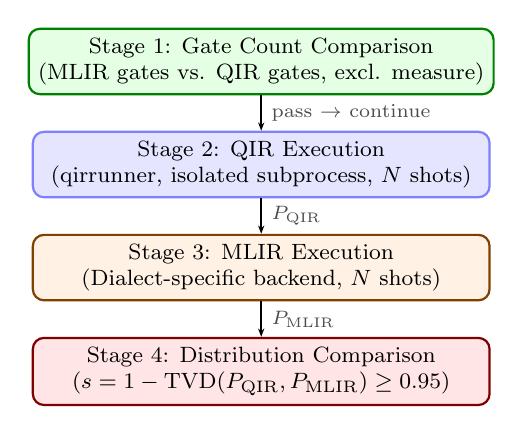
\begin{tikzpicture}[
    node distance=0.45cm,
    stage/.style={draw, rounded corners, minimum height=0.7cm, minimum width=5.8cm, align=center, font=\footnotesize, thick},
    s1/.style={stage, fill=green!10, draw=green!50!black},
    s2/.style={stage, fill=blue!10, draw=blue!50},
    s3/.style={stage, fill=orange!10, draw=orange!50!black},
    s4/.style={stage, fill=red!10, draw=red!50!black},
    arrow/.style={-{Stealth[length=3pt]}, thick},
    lbl/.style={font=\scriptsize, text=gray!60!black},
]
\node[s1] (s1) {Stage 1: Gate Count Comparison\\(MLIR gates vs. QIR gates, excl. measure)};
\node[s2, below=of s1] (s2) {Stage 2: QIR Execution\\(qirrunner, isolated subprocess, $N$ shots)};
\node[s3, below=of s2] (s3) {Stage 3: MLIR Execution\\(Dialect-specific backend, $N$ shots)};
\node[s4, below=of s3] (s4) {Stage 4: Distribution Comparison\\($s = 1 - \text{TVD}(P_\text{QIR}, P_\text{MLIR}) \geq 0.95$)};

\draw[arrow] (s1) -- node[lbl, right] {pass $\rightarrow$ continue} (s2);
\draw[arrow] (s2) -- node[lbl, right] {$P_\text{QIR}$} (s3);
\draw[arrow] (s3) -- node[lbl, right] {$P_\text{MLIR}$} (s4);
\end{tikzpicture}
\caption{Four-stage dual-backend verification pipeline. Each stage provides progressively deeper correctness assurance, from structural gate comparison to distributional equivalence via TVD.}
\label{fig:verification}
\end{figure}

\textbf{Stage 1: Gate count comparison.} The system independently counts gates in the original MLIR and the generated QIR. For MLIR, gate names are extracted from \texttt{quantum.custom} (Catalyst) or dialect-specific operations (Quake) and normalized to lowercase canonical names. For QIR, gate names are extracted from \texttt{call void @\_\_quantum\_\_qis\_\_<gate>\_\_body} patterns. Measurement operations are excluded from both counts because they are infrastructure operations injected at verification time rather than unitary gates specified by the circuit designer. A gate count mismatch provides an immediate signal that the translation introduced or dropped operations.

\textbf{Stage 2: QIR execution.} The generated QIR is executed using the \texttt{qirrunner} package (version 0.9.1), which provides a Python interface to a QIR execution engine. To avoid conflicts between the LLVM libraries linked by \texttt{qirrunner} and the JAX/XLA runtime used by PennyLane Catalyst, execution is performed in an isolated subprocess. Before execution, a preprocessing step ensures that measurement operations cover all qubits in the circuit and that output recording calls are present in the correct order. The executor runs the circuit for $N$ shots (default $N=1024$) and parses the output into a bitstring frequency distribution $P_{\text{QIR}}$.

\textbf{Stage 3: MLIR execution.} The original MLIR circuit is independently executed on a dialect-specific backend selected through an extensible simulator registry. For the Catalyst dialect, the system reconstructs a PennyLane quantum node (\texttt{QNode}) from the parsed circuit, applies the \texttt{@catalyst.qjit} just-in-time compiler with the \texttt{lightning.qubit} simulator~\cite{bergholm2022pennylane}, and collects measurement samples. For circuits containing mid-circuit measurements (conditional operations), the system uses a snapshot-based construction approach that replays gate sequences inside the JIT-compiled function using Catalyst's \texttt{@catalyst.cond} decorator for branching. For the Quake dialect, the system uses CUDA Quantum~\cite{kim2023cudaquantum} as the execution backend, constructing a kernel via \texttt{cudaq.make\_kernel()} and sampling with \texttt{cudaq.sample()}. Both backends execute in isolated subprocesses to avoid LLVM library conflicts. The registry pattern allows additional backends to be registered for new dialects; for unseen dialects where no backend is yet available, the pipeline falls back to QIR-only verification (Stages~1, 2, and~4 with the QIR-side distribution only). The execution produces a second bitstring frequency distribution $P_{\text{MLIR}}$.

\textbf{Stage 4: Distribution comparison.} The two output distributions are compared using the total variation distance (TVD), defined as:

\begin{equation}
\text{TVD}(P, Q) = \frac{1}{2} \sum_{x \in \mathcal{X}} |P(x) - Q(x)|
\label{eq:tvd}
\end{equation}

\noindent where $\mathcal{X}$ is the set of all observed bitstring outcomes across both distributions, and $P(x)$ and $Q(x)$ are the empirical probabilities of outcome $x$ under each distribution. The TVD ranges from 0 (identical distributions) to 1 (completely disjoint support). We convert TVD to a similarity score $s = 1 - \text{TVD}$ and apply a pass threshold of $\tau = 0.95$, meaning the translation is accepted when the output distributions agree to within 5\% total variation. This threshold accounts for finite sampling noise inherent in shot-based simulation while remaining sensitive to gate errors that would produce qualitatively different output states.

We choose TVD over Kullback-Leibler (KL) divergence for two reasons. First, TVD is symmetric, which avoids the arbitrary choice of which distribution serves as the reference. Second, TVD is well-defined even when one distribution assigns zero probability to an outcome observed in the other, whereas KL divergence diverges in this case unless smoothing is applied.

\subsection{Guardrail-Assembler Pattern for LLM Output Recovery}\label{sec:guardrail}

Smaller LLMs (8B to 13B parameters) frequently produce output that contains the correct quantum operations but lacks the structural scaffolding required for valid QIR. Common failure modes include omitting type definitions (\texttt{\%Qubit = type opaque}), function declarations, attribute sections, and QIR metadata. In some cases, models emit a JSON object with an operations list rather than raw LLVM IR, or they produce tool-call JSON when confused by the agent framework's tool-use protocol.

To recover valid QIR from these partial outputs, we introduce a guardrail-assembler pattern that operates as a post-processing stage after each LLM invocation. The guardrail applies a cascade of five checks in order of priority, as shown in Fig.~\ref{fig:guardrail}.

\begin{figure}[htbp]
\centering
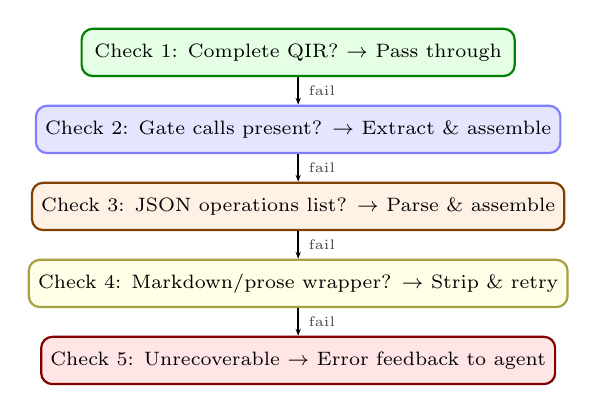
\begin{tikzpicture}[
    node distance=0.35cm,
    box/.style={draw, rounded corners, minimum height=0.6cm, minimum width=5.5cm, align=center, font=\scriptsize, thick},
    c1/.style={box, fill=green!10, draw=green!50!black},
    c2/.style={box, fill=blue!10, draw=blue!50},
    c3/.style={box, fill=orange!10, draw=orange!50!black},
    c4/.style={box, fill=yellow!10, draw=yellow!60!black},
    c5/.style={box, fill=red!10, draw=red!50!black},
    arrow/.style={-{Stealth[length=2.5pt]}, thick},
    lbl/.style={font=\tiny, text=gray!60!black},
]
\node[c1] (c1) {Check 1: Complete QIR? $\rightarrow$ Pass through};
\node[c2, below=of c1] (c2) {Check 2: Gate calls present? $\rightarrow$ Extract \& assemble};
\node[c3, below=of c2] (c3) {Check 3: JSON operations list? $\rightarrow$ Parse \& assemble};
\node[c4, below=of c3] (c4) {Check 4: Markdown/prose wrapper? $\rightarrow$ Strip \& retry};
\node[c5, below=of c4] (c5) {Check 5: Unrecoverable $\rightarrow$ Error feedback to agent};

\draw[arrow] (c1) -- node[lbl, right] {fail} (c2);
\draw[arrow] (c2) -- node[lbl, right] {fail} (c3);
\draw[arrow] (c3) -- node[lbl, right] {fail} (c4);
\draw[arrow] (c4) -- node[lbl, right] {fail} (c5);
\end{tikzpicture}
\caption{Guardrail-assembler cascade. Each check attempts to extract valid gate operations from the LLM output using progressively more aggressive parsing strategies.}
\label{fig:guardrail}
\end{figure}

The deterministic QIR assembler accepts a list of parsed gate operations and produces syntactically complete LLVM IR by instantiating the same templates used by the deterministic translation path. It normalizes gate names through an alias table that maps common LLM variants (e.g., ``hadamard'', ``cx'', ``pauli\_x'') to canonical QIR function suffixes, infers the qubit count from the maximum qubit index referenced in the operations, and automatically appends measurement operations for all qubits, output recording calls, function declarations, attributes, and QIR version metadata. This design ensures that any LLM output containing correct gate operations, regardless of formatting deficiencies, can be recovered into executable QIR.

\subsection{Context Engineering for LLM Translation}\label{sec:context}

Traditional approaches to providing domain knowledge to LLM agents rely on retrieval-augmented generation (RAG)~\cite{lewis2020rag}, in which relevant documents are retrieved from a vector database and injected into the prompt at query time. In preliminary experiments, we found that smaller models (8B parameters) frequently failed to use the retrieval tool correctly, issuing repeated identical queries or misinterpreting retrieved content. We therefore adopted a context engineering strategy in which all necessary reference material is injected directly into the task prompt.

The inline reference consists of three components: (1) a gate mapping table that associates each MLIR gate name with its QIR intrinsic function signature (Table~\ref{tab:gate_mapping}), covering single-qubit gates, parameterized rotation gates, and two-qubit gates; (2) a complete QIR example showing a two-qubit Bell state circuit with all required sections (header, entry function, declarations, attributes, and metadata); and (3) a set of translation pattern descriptions covering qubit allocation, gate sequencing, measurement recording, and conditional operations.

This approach increases prompt length but eliminates the retrieval failure mode entirely. Since the gate mapping table and QIR template are compact (approximately 2,000 tokens), the overhead is acceptable even for models with 4,096-token context windows. For unseen dialects where the inline reference may be insufficient, the agent retains access to a web search tool that can fetch external documentation.

\subsection{Multi-Model Support}\label{sec:models}

The system supports multiple LLM backends through a unified configuration layer. Local models are served through Ollama, supporting Llama 3.1~\cite{dubey2024llama3} (8B and 70B variants) and Code Llama~\cite{roziere2023codellama} (13B and 34B variants). Cloud-hosted models are accessed through the HuggingFace Inference API. The CrewAI agent framework~\cite{hong2024crewai} wraps the selected model in a unified interface for prompt formatting and ReAct~\cite{yao2023react} reasoning.

\section{Experimental Setup}\label{sec:experiments}

% Experiment headings are provided; results to be populated after data collection.
\subsection{Benchmark Circuits}

We assembled a benchmark suite of 39 unique quantum circuits spanning nine categories, with each circuit available in both Catalyst and Quake MLIR dialects where applicable. Table~\ref{tab:circuits} summarizes the benchmark. GHZ circuits provide a controlled scaling ladder from 4 to 100 qubits across 20 sizes (every 5 qubits from 5 to 100, plus 4) with identical gate structure (one Hadamard followed by $N{-}1$ CNOT gates). Measurement-based quantum computing (MBQC) circuits test conditional handling with mid-circuit measurements and classical feed-forward corrections. Random circuits stress-test gate diversity with mixed gate sets including rotations (RX, RY, RZ), phase gates (S, T), and two-qubit entangling operations (CZ, SWAP). The Steane code circuit is an error-correcting code pattern with 7 qubits and 10 CNOT gates. Four FTQC circuits written in an unseen dialect exercise the agentic translation path on Steane-encoded logical operations.

\begin{table*}[t]
\centering
\caption{Benchmark circuit suite (39 unique circuits). Circuits are organized by category with qubit counts, gate types, dialect availability, and count of distinct circuits per row.}
\label{tab:circuits}
\renewcommand{\arraystretch}{1.1}
\begin{tabular}{@{}llclll@{}}
\toprule
\textbf{Category} & \textbf{Circuit} & \textbf{Qubits} & \textbf{Key Gates} & \textbf{Dialects} & \textbf{Count} \\
\midrule
\multirow{2}{*}{Standard}   & Bell state         & 2   & H, CNOT       & Both (Catalyst \& Quake) & 1 \\
                             & GHZ-3              & 3   & H, CNOT$\times$2   & Both & 1 \\
\midrule
GHZ scaling & GHZ-\{5, 10, 15, ..., 100\} & 5--100 & H, CNOT$\times(N{-}1)$ & Both & 20 \\
\midrule
\multirow{2}{*}{MBQC}       & Teleport, RZ rotation  & 2   & H, CZ, X, conditional  & Both & 2 \\
                             & RX rotation, CNOT      & 3--4 & H, CZ, X, Z, conditional & Both & 2 \\
\midrule
Conditional                  & Classic teleportation  & 3   & H, CNOT, X, Z & Both & 1 \\
\midrule
Random                       & 5 mixed-gate circuits  & 2--7 & T, S, RX, RY, RZ, CZ, SWAP & Both & 5 \\
\midrule
QEC                          & Steane code            & 7   & H$\times$10, CNOT$\times$9 & Catalyst only & 1 \\
\midrule
Parametric                   & RX/RY/RZ rotations     & 1   & RX, RY, RZ    & Catalyst only & 1 \\
\midrule
Variational                  & Autodiff gradient      & 1   & RX, ExpVal(PauliZ)    & Catalyst only & 1 \\
\midrule
\multirow{2}{*}{FTQC (unseen)} & Steane 1Q H, 2Q Bell & 1--2\textsuperscript{$\dagger$} & Logical H, CNOT & FTQC only & 2 \\
                             & Steane 3Q Grover, 3Q QFT & 3\textsuperscript{$\dagger$}   & Logical H, CZ, Z & FTQC only & 2 \\
\midrule
\multicolumn{5}{@{}r}{\textbf{Total unique circuits}} & \textbf{39} \\
\bottomrule
\multicolumn{6}{@{}l}{\footnotesize \textsuperscript{$\dagger$}Logical qubits; physical count is $7\times$ under Steane [[7,1,3]] encoding.}
\end{tabular}
\end{table*}

For GHZ circuits at sizes 30 and 100, we generated independent QIR ground-truth files via the \texttt{qiskit-qir} package from equivalent Qiskit \texttt{QuantumCircuit} objects, providing a third-party reference for structural comparison. The FTQC circuits use a custom \texttt{ftqc} dialect with Steane-encoded logical qubit operations (\texttt{ftqc.init\_zero}, \texttt{ftqc.logical\_h}, \texttt{ftqc.logical\_cnot}), which is not registered in the deterministic parser. These circuits exercise the agentic translation path on a genuinely unseen dialect.


\subsection{Models Under Test}

We evaluated five LLM models spanning three size classes and two architectures (Table~\ref{tab:models}). All local models were served through Ollama; the cloud model accessed the HuggingFace Inference API. The deterministic parser (no LLM) served as the baseline for all comparisons.

\begin{table}[htbp]
\centering
\caption{LLM models evaluated. VRAM listed for local Ollama deployment.}
\label{tab:models}
\renewcommand{\arraystretch}{1.1}
\begin{tabular}{@{}llcl@{}}
\toprule
\textbf{Model} & \textbf{Provider} & \textbf{Params} & \textbf{VRAM} \\
\midrule
Llama 3.1      & Ollama (local)     & 8B   & $\sim$6~GB  \\
Llama 3.1      & Ollama (local)     & 70B  & $\sim$40~GB \\
Code Llama     & Ollama (local)     & 13B  & $\sim$8~GB  \\
Code Llama     & Ollama (local)     & 34B  & $\sim$20~GB \\
GPT-OSS-20B    & HuggingFace (API)  & 20B  & Cloud       \\
\bottomrule
\end{tabular}
\end{table}
\subsection{Evaluation Metrics}

We report four primary metrics across experiments:

\begin{itemize}
    \item \textbf{Gate match rate}: Binary correctness of gate-level translation. The MLIR and QIR gate counts (excluding measurement operations) must be identical in type and quantity.
    \item \textbf{TVD similarity}: $s = 1 - \text{TVD}(P_\text{QIR}, P_\text{MLIR})$, measured in two modes: \emph{shots mode} (1,024 samples per backend, both sides subject to sampling noise) and \emph{probs mode} (exact probabilities from MLIR-side state vector via \texttt{qml.probs()}, 100K shots on QIR side). The probs mode isolates translation errors from sampling noise.
    \item \textbf{Translation time}: Wall-clock time from MLIR input to QIR output, excluding verification.
    \item \textbf{Iteration count}: Number of agent refinement iterations before convergence (1 for deterministic path).
\end{itemize}


\subsection{Hardware and Software Configuration}

All experiments were conducted on a workstation equipped with an NVIDIA RTX 6000 Ada GPU (48~GB VRAM), Intel Xeon w5-2465X processor, and 256~GB RAM, running Ubuntu 22.04. Software versions: Python~3.12, PennyLane~0.44.0, PennyLane-Catalyst~0.14.0, CUDA Quantum~0.13, \texttt{qirrunner}~0.9.1, CrewAI~1.10.0, Ollama~0.6. We note that \texttt{qirrunner} and CrewAI are under active development; API changes in future releases may require minor adaptation. Each agentic experiment was repeated 3 times to capture LLM output variance.


\section{Results}\label{sec:results}

\subsection{Translation Correctness (E1)}

Table~\ref{tab:e1} reports the deterministic translation results across both dialects and verification modes. The benchmark includes 37 Catalyst circuits and 35 Quake circuits, for a total of 72 dialect-circuit pairs. Of these, 71 achieve correct gate-level translation; the single failure is a Quake-dialect Bell state file misrouted through the Catalyst parser due to its placement in a generic examples directory rather than the dialect-specific directory. Circuits with 35 or more qubits are translated and gate-checked but excluded from TVD statistics because the $2^N$-dimensional state vector exceeds available memory for simulation. Among the 38 circuit pairs where both backends could be executed, TVD similarity averages 97.9\% in shots mode and 98.8\% in probs mode. The gap between modes confirms that the residual TVD shortfall under shots mode is attributable to finite sampling noise rather than translation error. Three circuits (two random circuits and one conditional circuit) exhibit gate-level matches but produce divergent simulation distributions (TVD near 0\%), which we attribute to mid-circuit measurement semantics that the MLIR-side executor does not fully reconstruct; these are discussed in Section~\ref{sec:limitations}.

\begin{table}[htbp]
\centering
\caption{E1: Deterministic translation correctness. Gate match rate and TVD similarity across dialects and verification modes. Circuits $\geq$35 qubits are gate-checked only (TVD requires state-vector simulation). Three circuits with known simulation divergence and one misrouted dialect file are excluded from TVD averages.}
\label{tab:e1}
\renewcommand{\arraystretch}{1.1}
\begin{tabular}{@{}lcccccc@{}}
\toprule
\textbf{Dialect} & \textbf{Mode} & \textbf{Total} & \textbf{Gate OK} & \textbf{TVD $n$} & \textbf{Avg} & \textbf{Min} \\
\midrule
Catalyst & Shots & 37 & 36 & 20 & 97.7\% & 91.3\% \\
Catalyst & Probs & 37 & 36 & 20 & 99.3\% & 96.3\% \\
Quake    & Shots & 35 & 35 & 18 & 98.2\% & 93.4\% \\
Quake    & Probs & 35 & 35 & 18 & 98.4\% & 93.8\% \\
\bottomrule
\end{tabular}
\end{table}

\subsection{Scalability (E2)}

To assess how translation quality scales with circuit size, we evaluated GHZ circuits across seven sizes (5, 10, 15, 20, 25, and 30 qubits with full TVD verification, plus 100 qubits with gate checking only) in both Catalyst and Quake dialects. All 16 circuit-dialect pairs achieve 100\% gate match. Deterministic translation time remains below 25~ms across all sizes, confirming O($n$) scaling with respect to gate count. Among the 14 pairs where TVD could be computed (GHZ-5 through GHZ-30, both dialects), shots-mode TVD averages 98.5\% with a minimum of 96.2\%, and probs-mode TVD averages 99.4\% with a minimum of 97.3\%. GHZ-100 is correctly translated (100 gates, verified by structural comparison against an independent Qiskit-generated QIR reference) but cannot be simulated on 256~GB RAM.

\subsection{Cross-Dialect Portability (E6)}

To test whether the system produces semantically equivalent QIR regardless of input dialect, we translated 14 matched Catalyst--Quake circuit pairs through the deterministic path and compared the outputs. All 14 pairs achieve gate-level match in both dialects. For the 11 pairs where TVD could be computed on both sides, Catalyst-side TVD averages 99.4\% and Quake-side TVD averages 98.5\%, both in probs mode. Two random circuits (\texttt{random\_1847} and \texttt{random\_2449}) produce TVD near 0\% despite correct gate counts, the same simulation-divergence issue observed in E1. GHZ-100 is gate-matched on both sides but excluded from TVD comparison.

\subsection{Unseen Dialect Translation (E7)}

To evaluate extensibility beyond the two registered dialects, we tested the agentic path on four circuits written in a custom FTQC dialect that encodes logical qubits using the Steane [[7,1,3]] error-correcting code. The FTQC dialect uses operations such as \texttt{ftqc.init\_zero} and \texttt{ftqc.logical\_h} that have no entry in the deterministic parser's gate table. When the system encounters this dialect, it identifies the \texttt{ftqc} namespace as unknown and routes the circuit to the agentic translation path, equipping the LLM agent with web search and simulator discovery tools.

Table~\ref{tab:e7} reports the results. The deterministic path rejects all four circuits with exit code~2 (unsupported dialect), confirming correct routing. Llama~3.1 (8B) produces valid QIR for all four circuits on the first iteration, mapping each logical FTQC operation to its QIR counterpart (e.g., \texttt{ftqc.logical\_h} $\to$ \texttt{@\_\_quantum\_\_qis\_\_h\_\_body}). Code Llama (13B) succeeds on the two simpler circuits but fails on the three-qubit Grover and QFT circuits, emitting tool-call JSON instead of LLVM IR. This failure mode is specific to code-specialized models whose tool-use training interferes with direct output generation in the CrewAI agent framework.

\begin{table}[htbp]
\centering
\caption{E7: Unseen dialect (FTQC) translation. Success indicates valid QIR produced; logical gates lists the gate calls in the generated QIR. No MLIR backend exists for FTQC, so TVD verification is not applicable. Each circuit was run 3 times per model.}
\label{tab:e7}
\renewcommand{\arraystretch}{1.1}
\begin{tabular}{@{}llccc@{}}
\toprule
\textbf{Circuit} & \textbf{Model} & \textbf{Success} & \textbf{Iter.} & \textbf{Logical Gates} \\
\midrule
\multirow{2}{*}{1Q Hadamard}  & Llama 3.1 (8B)   & 3/3 & 1 & H, mz \\
                               & Code Llama (13B)  & 3/3 & 1 & H, mz \\
\midrule
\multirow{2}{*}{2Q Bell}      & Llama 3.1 (8B)   & 3/3 & 1 & H, CNOT, 2$\times$mz \\
                               & Code Llama (13B)  & 3/3 & 1 & H, CNOT, 2$\times$mz \\
\midrule
\multirow{2}{*}{3Q Grover}    & Llama 3.1 (8B)   & 3/3 & 1 & 2H, 2CNOT, 6$\times$mz \\
                               & Code Llama (13B)  & 0/3 & -- & (tool-call JSON) \\
\midrule
\multirow{2}{*}{3Q QFT}       & Llama 3.1 (8B)   & 3/3 & 1 & 3H, 2CNOT, CZ \\
                               & Code Llama (13B)  & 0/3 & -- & (tool-call JSON) \\
\bottomrule
\end{tabular}
\end{table}

The generated QIR represents a logical-level translation: the LLM correctly identifies the gate semantics of the FTQC operations but does not expand them into the physical Steane encoding, which would require 7 transversal gates per logical operation and a 12-gate encoding circuit per logical qubit. This distinction between logical and physical QIR is inherent to fault-tolerant quantum computing. In current FTQC compilation stacks, the error-correction encoding is typically the responsibility of the backend runtime rather than the IR, making the logical-level output a reasonable translation target.

\section{Discussion}\label{sec:discussion}

\subsection{Deterministic vs. Agentic Trade-offs}

The deterministic path translates recognized dialects in under 25~ms with near-perfect gate-level correctness (71/72 circuit pairs). The agentic path trades speed for generality: it handles unseen dialects at the cost of 5--15~seconds per translation and model-dependent output quality. The repair path (Path~3) combines both approaches, using the deterministic parser as a first attempt and falling back to LLM repair only when verification fails. In practice, the repair path is triggered by circuits whose conditional logic the deterministic parser handles structurally but that produce unexpected simulation behavior due to mid-circuit measurement semantics.

\subsection{Context Engineering vs. RAG}

Replacing RAG with inline context injection was driven by failure modes observed with 8B-parameter models. These models issued repeated identical retrieval queries, misinterpreted retrieved passages, or produced tool-call JSON instead of translation output. Injecting the gate mapping table and QIR template directly into the prompt ($\sim$2,000 tokens) eliminated retrieval failures while keeping the overhead within the context window of even small models. The agent retains access to web search tools for unseen dialects, though our experiments indicate that current models rarely use these tools without explicit instruction.

\subsection{Unseen Dialect Generalization}

The FTQC experiment (E7) shows that the system translates circuits from entirely new dialects without code changes. The LLM agent infers logical gate semantics from operation names alone (\texttt{ftqc.logical\_h} $\to$ Hadamard), producing valid QIR that captures the circuit's logical structure. The gap between logical-level and physical-level translation (Steane encoding expansion) reflects domain knowledge absent from the LLM's training data. An unexpected finding is that the general-purpose Llama~3.1 (8B) outperforms the code-specialized Code~Llama (13B) on this task: Code~Llama's tool-use training causes it to emit tool-call JSON rather than LLVM IR when processing unfamiliar dialects. Bridging the logical-to-physical gap could involve few-shot examples of error-correction encodings, domain-specific retrieval from QEC documentation, or models fine-tuned on fault-tolerant compilation patterns.

\subsection{Limitations}\label{sec:limitations}

Several limitations constrain the current evaluation. First, simulation-based verification requires $2^N$ memory for an $N$-qubit circuit; circuits with 35 or more qubits can only be gate-checked, not distribution-compared. Second, three circuits (\texttt{random\_1847}, \texttt{random\_2449}, and one conditional circuit) produce correct gate counts but divergent output distributions (TVD near 0\%). In each case, the MLIR-side executor does not fully reconstruct the mid-circuit measurement and classical feed-forward logic, leading to a mock or degenerate distribution. The QIR-side execution produces the expected output, indicating a limitation of the MLIR backend reconstruction rather than a translation error. Third, the autodiff gradient circuit is not supported in the verification pipeline because the MLIR-side executor does not reconstruct gradient computation graphs. Fourth, one Quake-dialect Bell state file placed in a generic directory was misrouted through the Catalyst parser, producing an empty QIR output; this is a file-organization issue rather than a parser defect. Fifth, for the unseen FTQC dialect, no MLIR backend is available, so verification is limited to structural inspection of the generated QIR. Finally, our benchmark covers two registered dialects and one unseen dialect; evaluation across additional MLIR dialects (OpenPulse, Quil, Stim) would test generalizability more broadly.

\section{Conclusion}\label{sec:conclusion}

We presented a hybrid system for MLIR-to-QIR translation that integrates deterministic compiler techniques with LLM-based agentic translation and iterative repair. The three-path architecture routes circuits through the fastest reliable path: deterministic parsing for known dialects, agentic translation for unseen dialects, and LLM-guided repair when verification fails. A dual-backend verification pipeline provides execution-based correctness checking by running source MLIR and target QIR on independent simulators and comparing output distributions via TVD.

On a 39-circuit benchmark spanning two registered dialects (Catalyst and Quake) and one unseen dialect (FTQC), with GHZ circuits scaling from 5 to 100 qubits across 20 sizes, the deterministic path achieved 98.6\% gate-level correctness (71/72 pairs) with TVD similarity averaging 97.9--99.3\% across 38 simulable circuit pairs. Cross-dialect evaluation on 14 matched Catalyst--Quake pairs confirmed gate-level equivalence in all cases. For the unseen FTQC dialect, the agentic path produced valid logical-level QIR for all four test circuits using Llama~3.1 (8B), demonstrating that the system generalizes to dialects absent from its deterministic parser.

Future work will extend the system along four axes: supporting additional MLIR dialects as they emerge in the quantum ecosystem, fine-tuning domain-specific LLMs on a corpus of quantum IR translations, integrating formal verification methods alongside simulation-based TVD checking, and extending the verification pipeline to support fault-tolerant encoding expansions and parameterized variational circuits.

\section*{Acknowledgment}

This work was supported by the U.S. Department of Energy, Office of Science under Contract No. DE-AC05-00OR22725, with funding from the Office of Advanced Scientific Computing Research's Accelerated Research in Quantum Computing Program's Modular and Error-Aware Software Stack for Heterogeneous Quantum Computing Ecosystems (MACH-Q) project.



\bibliographystyle{IEEEtran}
\bibliography{references}

\end{document}
